\section{Land Cover Semantic Segmentation}

\subsection{Data}
\begin{frame}{Data Acquisition}
    现阶段遥感图像语义分割数据集较多

    \begin{itemize}
        \item 建筑: Aerial Image Segmentation Dataset
        \item 道路: Massachusetts Roads Dataset
        \item 多类: GID
    \end{itemize}

    可惜GID的代码未开源
    
    只有数据集开源, 现已下载

\end{frame}

\begin{frame}{Gaofen Image Dataset}
    GID用高分2号数据做成的大范围土地利用覆盖数据集.

    \begin{figure}[!htbp]
        \centering
        \subfloat[input]{\label{fig:0201a}
        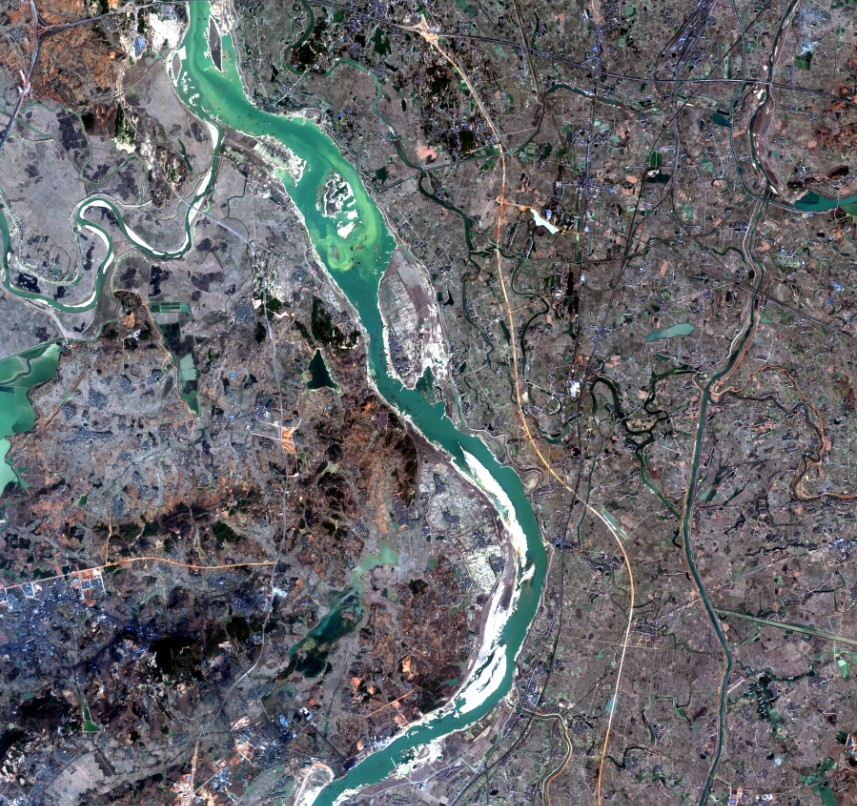
\includegraphics[height=4cm]{pic/pic0201a.jpg}}
        \quad
        \subfloat[output]{\label{fig:0201b}
        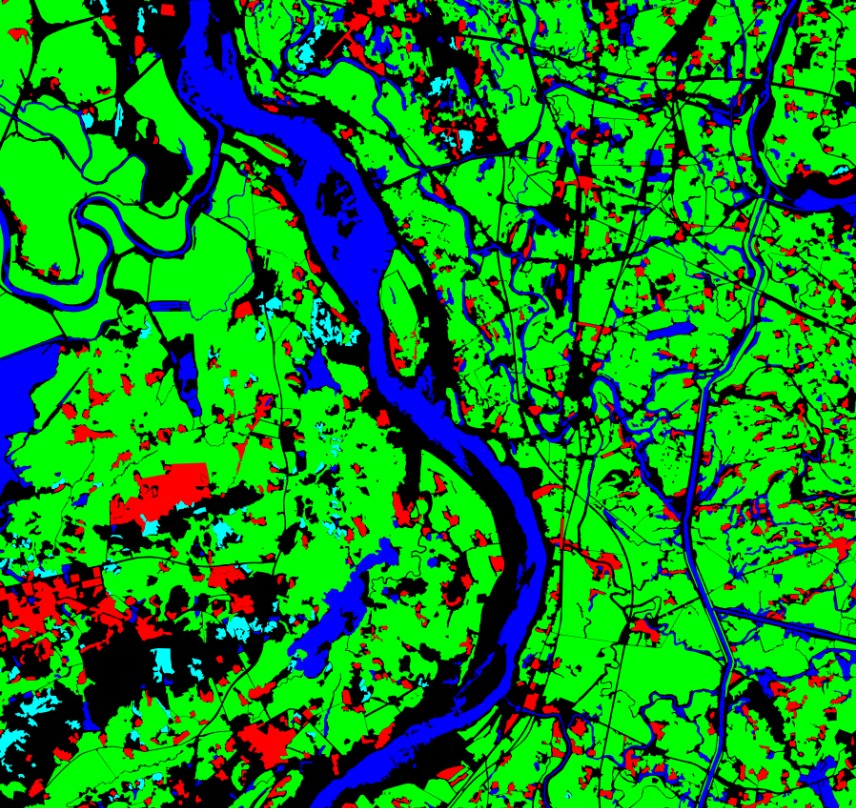
\includegraphics[height=4cm]{pic/pic0201b.jpg}}
        \caption{GID 数据}
        \label{fig:0201}
    \end{figure}
    
\end{frame}

\subsection{Method}
\begin{frame}{Method}
    对于如何得到影像分类结果:
    \begin{itemize}
        \item 输入影像如何得到分类结果
        \item 是否需要自己训练模型
        \item 预训练模型是否可以直接使用
    \end{itemize}    
    对于如何得到分类精度结果:
    \begin{itemize}
        \item 是否有开源代码可使用
    \end{itemize}
\end{frame}